\begin{frame}{Dischi di accrescimento: }
\begin{figure}[!ht]
	\begin{subfigure}[b]{0.39\textwidth}
		\centering
		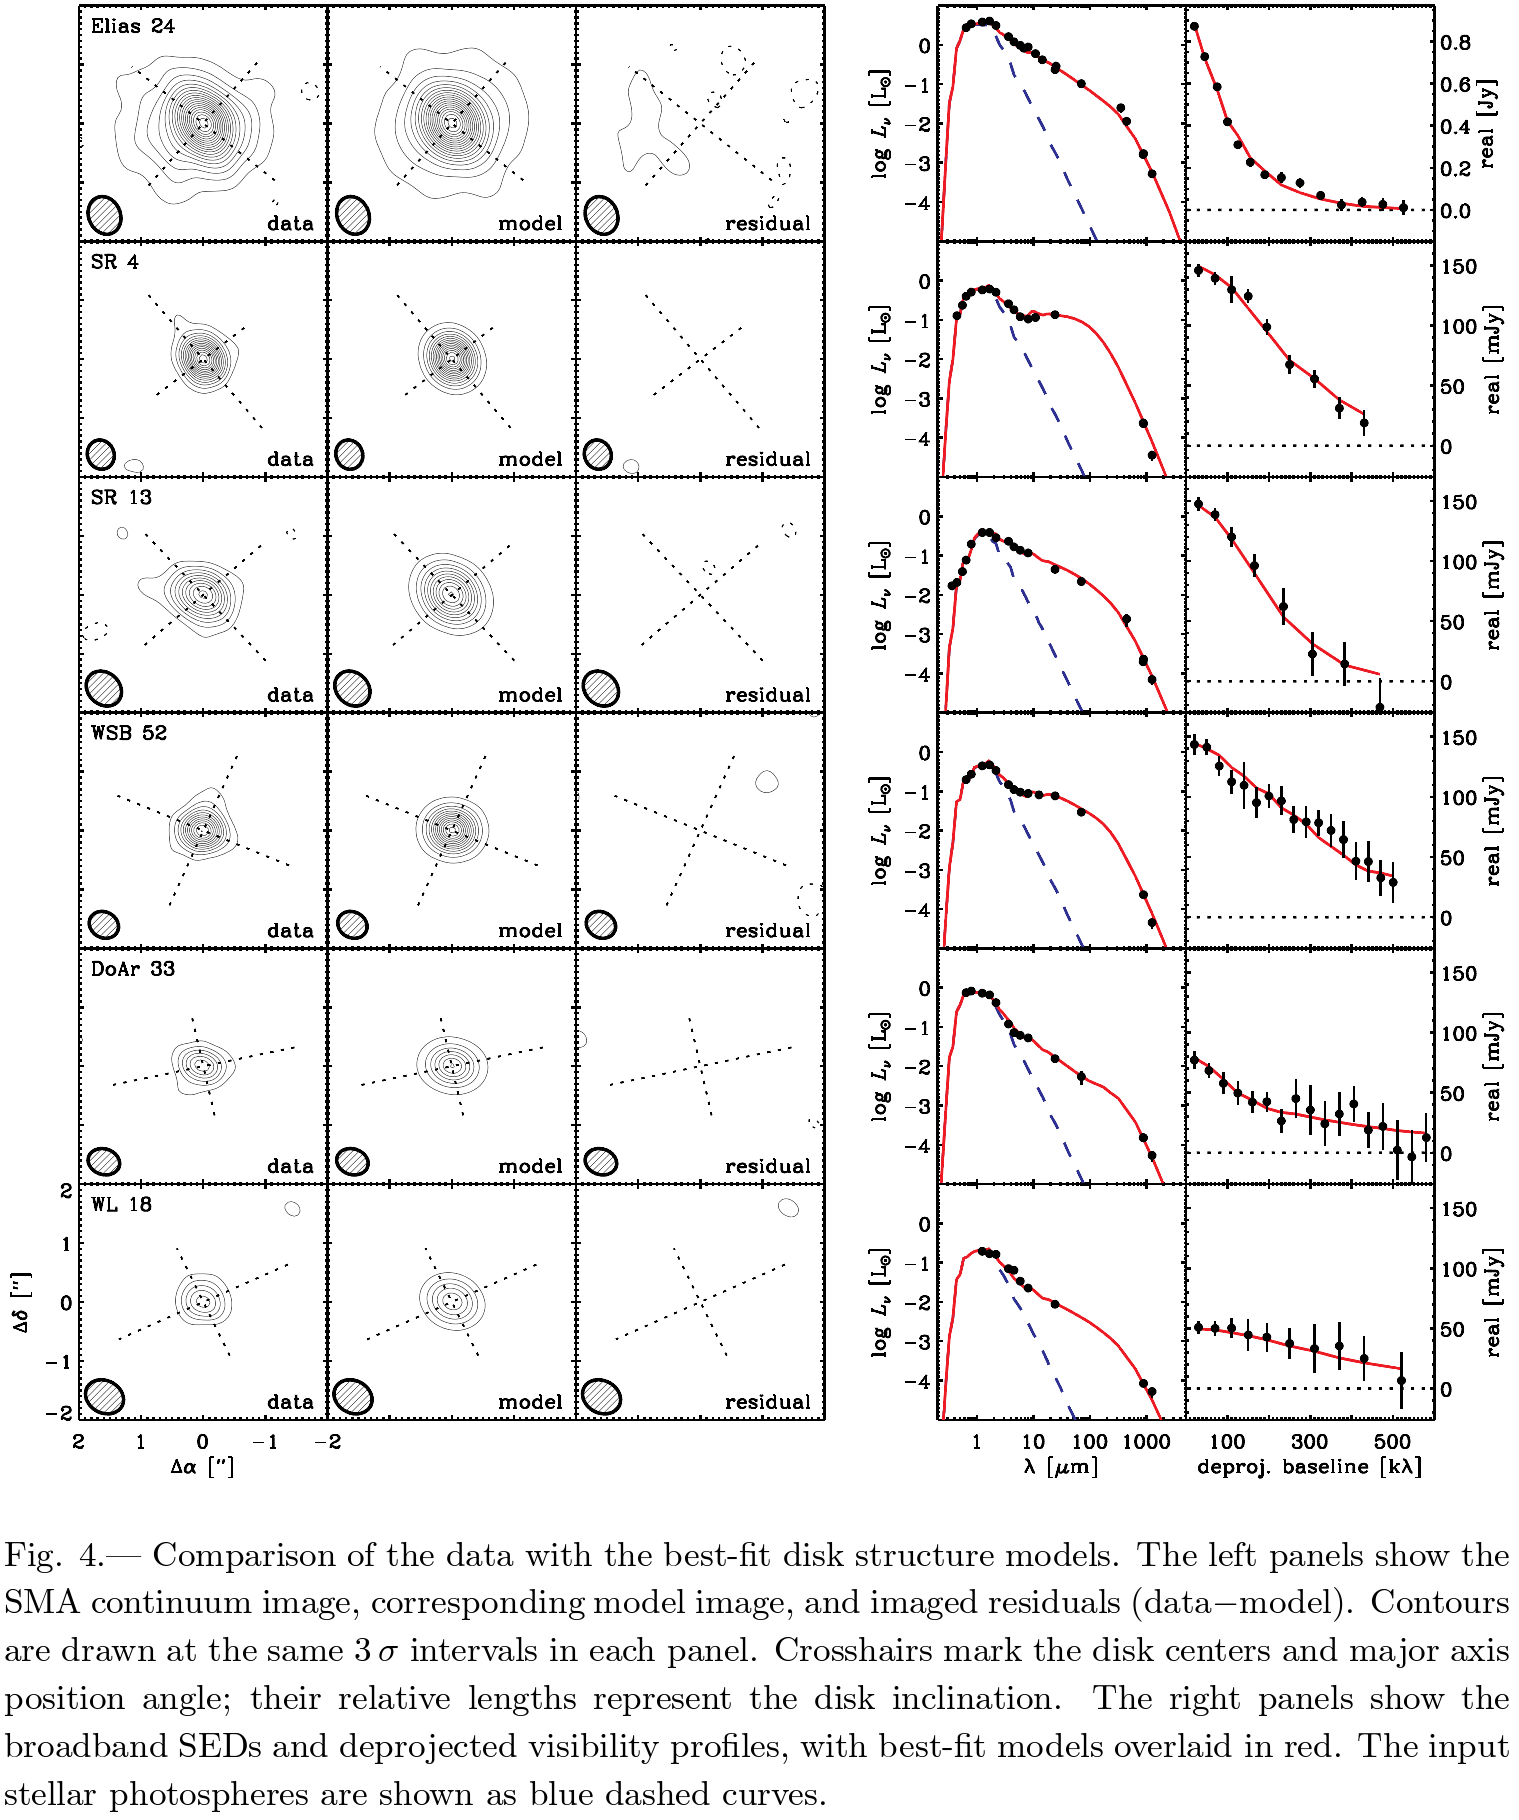
\includegraphics[trim={0cm 10cm 0 0},clip, keepaspectratio,width=0.98\textwidth]{SED-contours}
		\caption{Da \cite{andrews2010protoplanetary}.}\label{fig:SED-contours}
	\end{subfigure}
	~
	\begin{subfigure}[b]{0.55\textwidth}
		\centering
		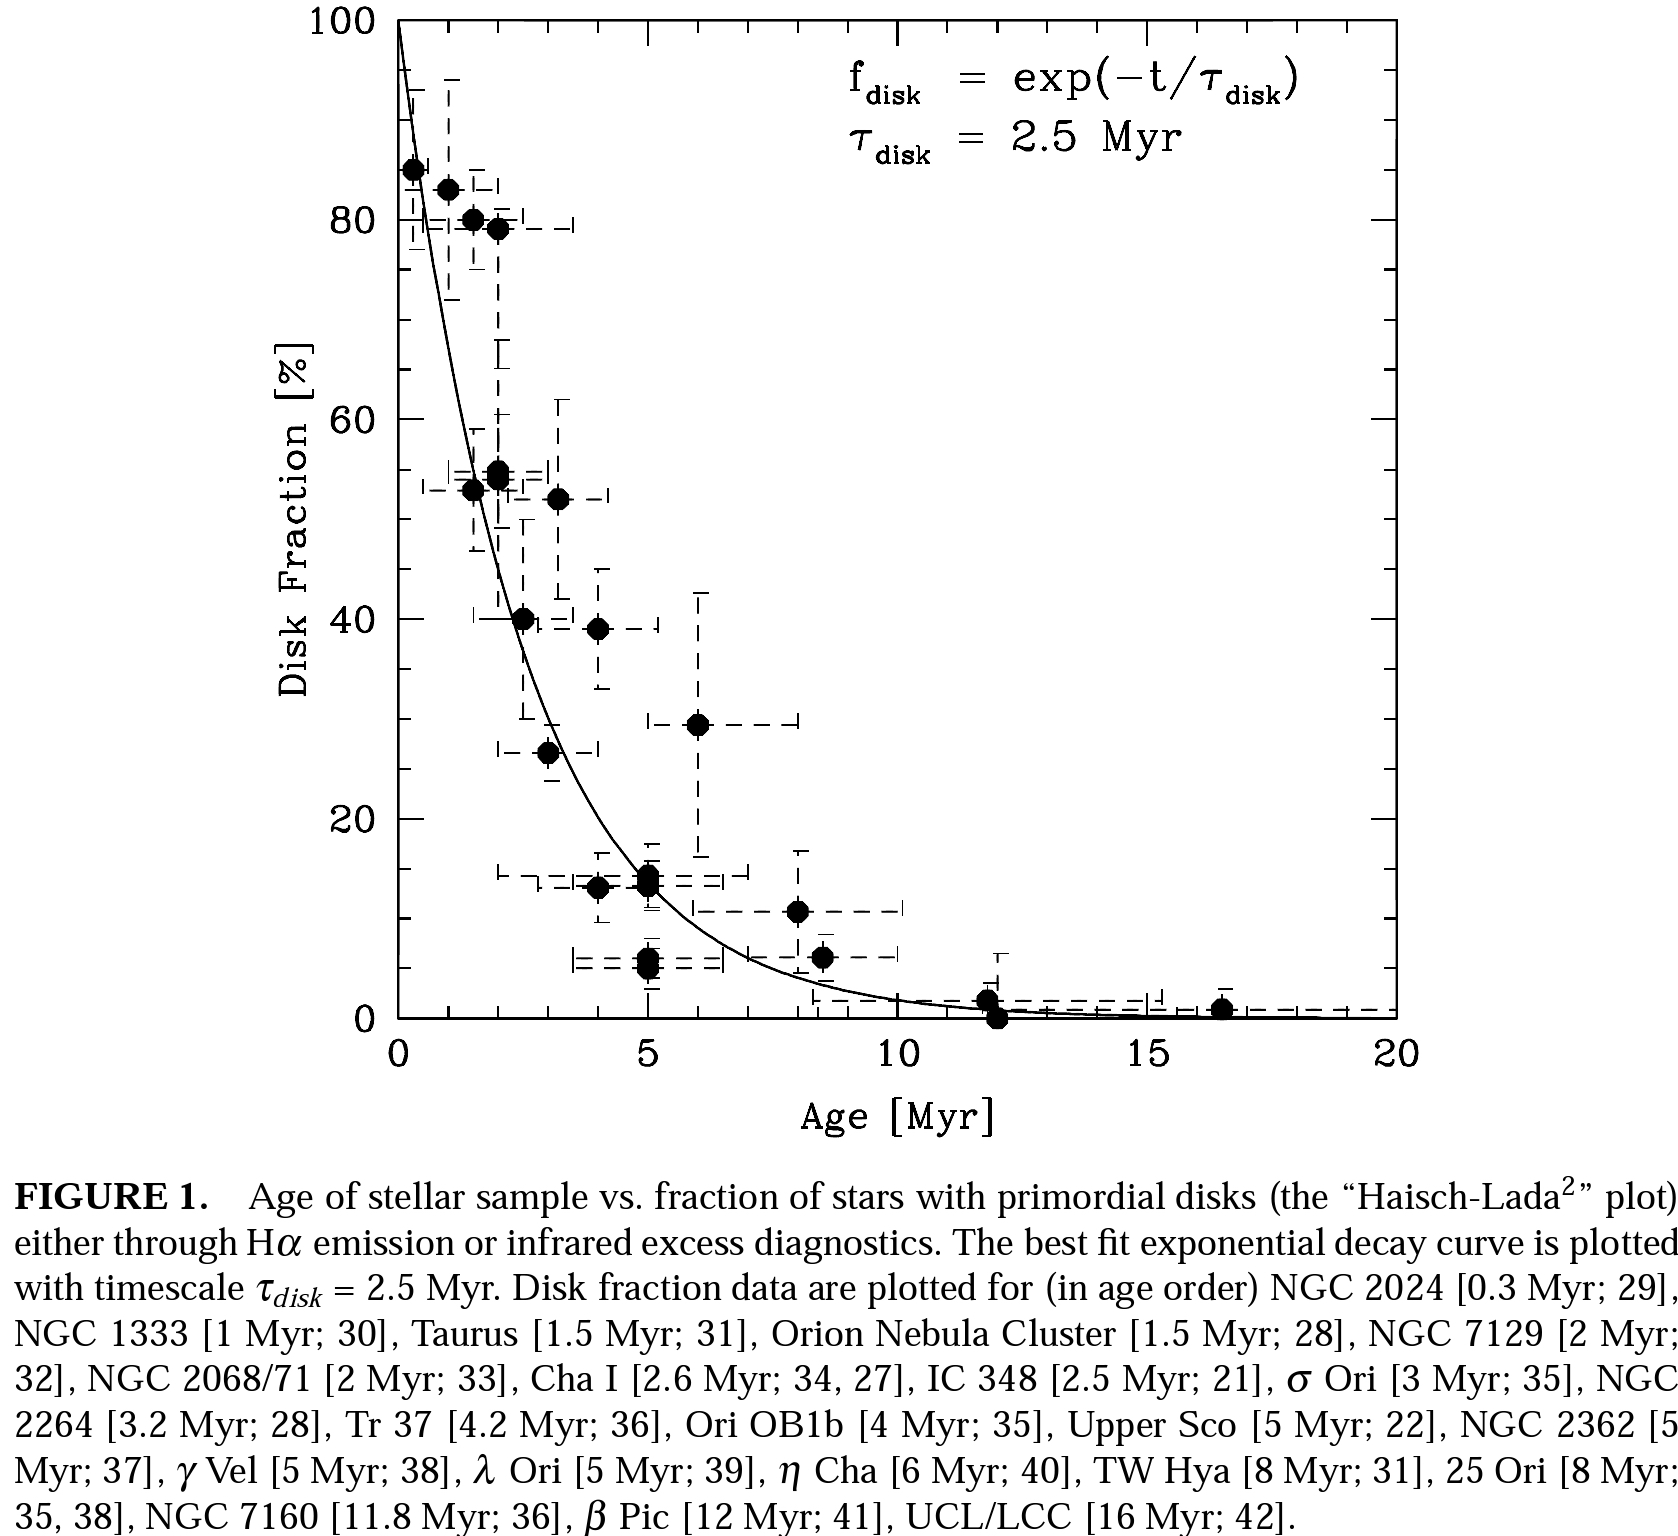
\includegraphics[trim={0cm 13cm 0 0},clip, width=0.99\textwidth,keepaspectratio]{clusterage-fstar}
		\caption{Da \cite{mamajek2009initial}. }\label{fig:clusterage-fstar}
	\end{subfigure}
\end{figure}
\begin{columns}[T]
\begin{column}{0.5\textwidth}
\begin{align*}
&\sigma_{r\phi}=\Sigma\nu r \TDy{r}{\Omega}\\
&\nu=\alpha c_sH
\end{align*}
\end{column}
\begin{column}{0.5\textwidth}
\begin{equation*}
\PDy{t}{\Sigma}=3\frac{1}{r}\PDof{r}[r\expy{1/2}\PDof{r}(\nu\Sigma r\expy{1/2})]\label{eq:sigmaevol}
\end{equation*}
\end{column}
\end{columns}
\end{frame}

\begin{frame}{Evoluzione del disco di polvere. Formazione dei nuclei solidi}

\begin{columns}[T]
\begin{column}{0.37\textwidth}
	\begin{block}{Sedimentazione e drag-forces}
\begin{align*}
&m_p\TDy{t}{\vec{v}}=\vec{F}_D-m_p\Omega^2z\hat{z}\\
&F_D=\frac{1}{2}C_D\pi s^2\rho_gv^2
\end{align*}
\end{block}
\end{column}
\begin{column}{0.63\textwidth}
\begin{block}{Raggiungimento scala chilometrica: planetesimi}
Modello di Goldreich-Ward: disco di polvere sottile instabile.

In assenza di sedimentazione: urti a 2 corpi. Ruolo duplice della turbolenza.
\end{block}
\end{column}
\end{columns}
\begin{block}{Accrescimento protopianeti}
\begin{columns}[T]
\begin{column}{0.5\textwidth}
		\begin{align*}
		&\TDy{t}{M_e}=\pi R_e^2\rho_{pl}v F_g\\
		&=A\pi R_e^2\Sigma_p\Omega F_g
		\end{align*}
\end{column}
\begin{column}{0.5\textwidth}
\begin{align*}
&v\approx\sqrt{e^2+i^2}v_K\\
&f(e,i)=4\frac{\Sigma_p}{m}\frac{ei}{\exv{e^2}\exv{i^2}}\Exp{-\frac{e^2}{\exv{e^2}}-\frac{i^2}{\exv{i^2}}}
\end{align*}
\end{column}
\end{columns}
\end{block}
\end{frame}

\begin{wordonframe}{Disco di polvere e formazione di nuclei solidi: planetesimi}
nel caso cammino libero medio delle molecole di gas sia maggiore delle dimensioni della particella $C_D=\frac{8}{3}\frac{v_{th}}{v_z}$ (Epstein drag) per particelle pi\'u grandi \'e funzione del numero di Reynold.
	dove si assume che eccentricit\'a e inclinazione seguano distribuzione di Rayleigh (\cite{ida1992n})
	$M_{iso}=0.066\mearth{}$ a 1AU densit\'a MMSN $\Sigma_p=\SI{10}{\gram\per\square\cm}$, $M_{iso}=1.36\mearth{}$ a 5AU densit\'a MMSN $\Sigma_p=\SI{3}{\gram\per\square\cm}$,
\end{wordonframe}

\begin{frame}{Fase accrescimento di gas}
\begin{columns}[T]
	\begin{column}{0.5\textwidth}
		\begin{figure}[!ht]
			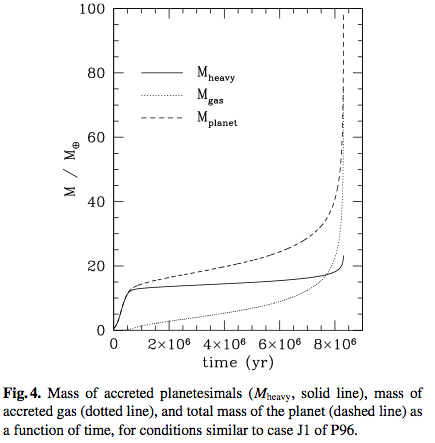
\includegraphics[trim={0cm 2cm 0 0},clip, keepaspectratio,width=0.98\textwidth]{massenvvscore}
			\caption{Da \cite{alibert2005models}.}\label{fig:massenvvscore}
		\end{figure}
	\end{column}
	\begin{column}{0.5\textwidth}
\begin{itemize}
	\item Accrescimento solidi runaway: $\frac{\dot{M}_e}{M_e}\propto M_e\expy{\frac{1}{3}}$
	\item Accrescimento gas su tempo scala $\tkh{}$
	\item Per $M_p\approx7-10\mearth{}$ crescita esponenziale dell'accrescimento di gas
	\item Accrescimento limitato da evoluzione viscosa del disco
\end{itemize}
\end{column}
\end{columns}
\end{frame}

\begin{frame}{Migrazione dei protopianeti}
\begin{columns}[T]
	\begin{column}{0.5\textwidth}
\begin{figure}[!ht]
	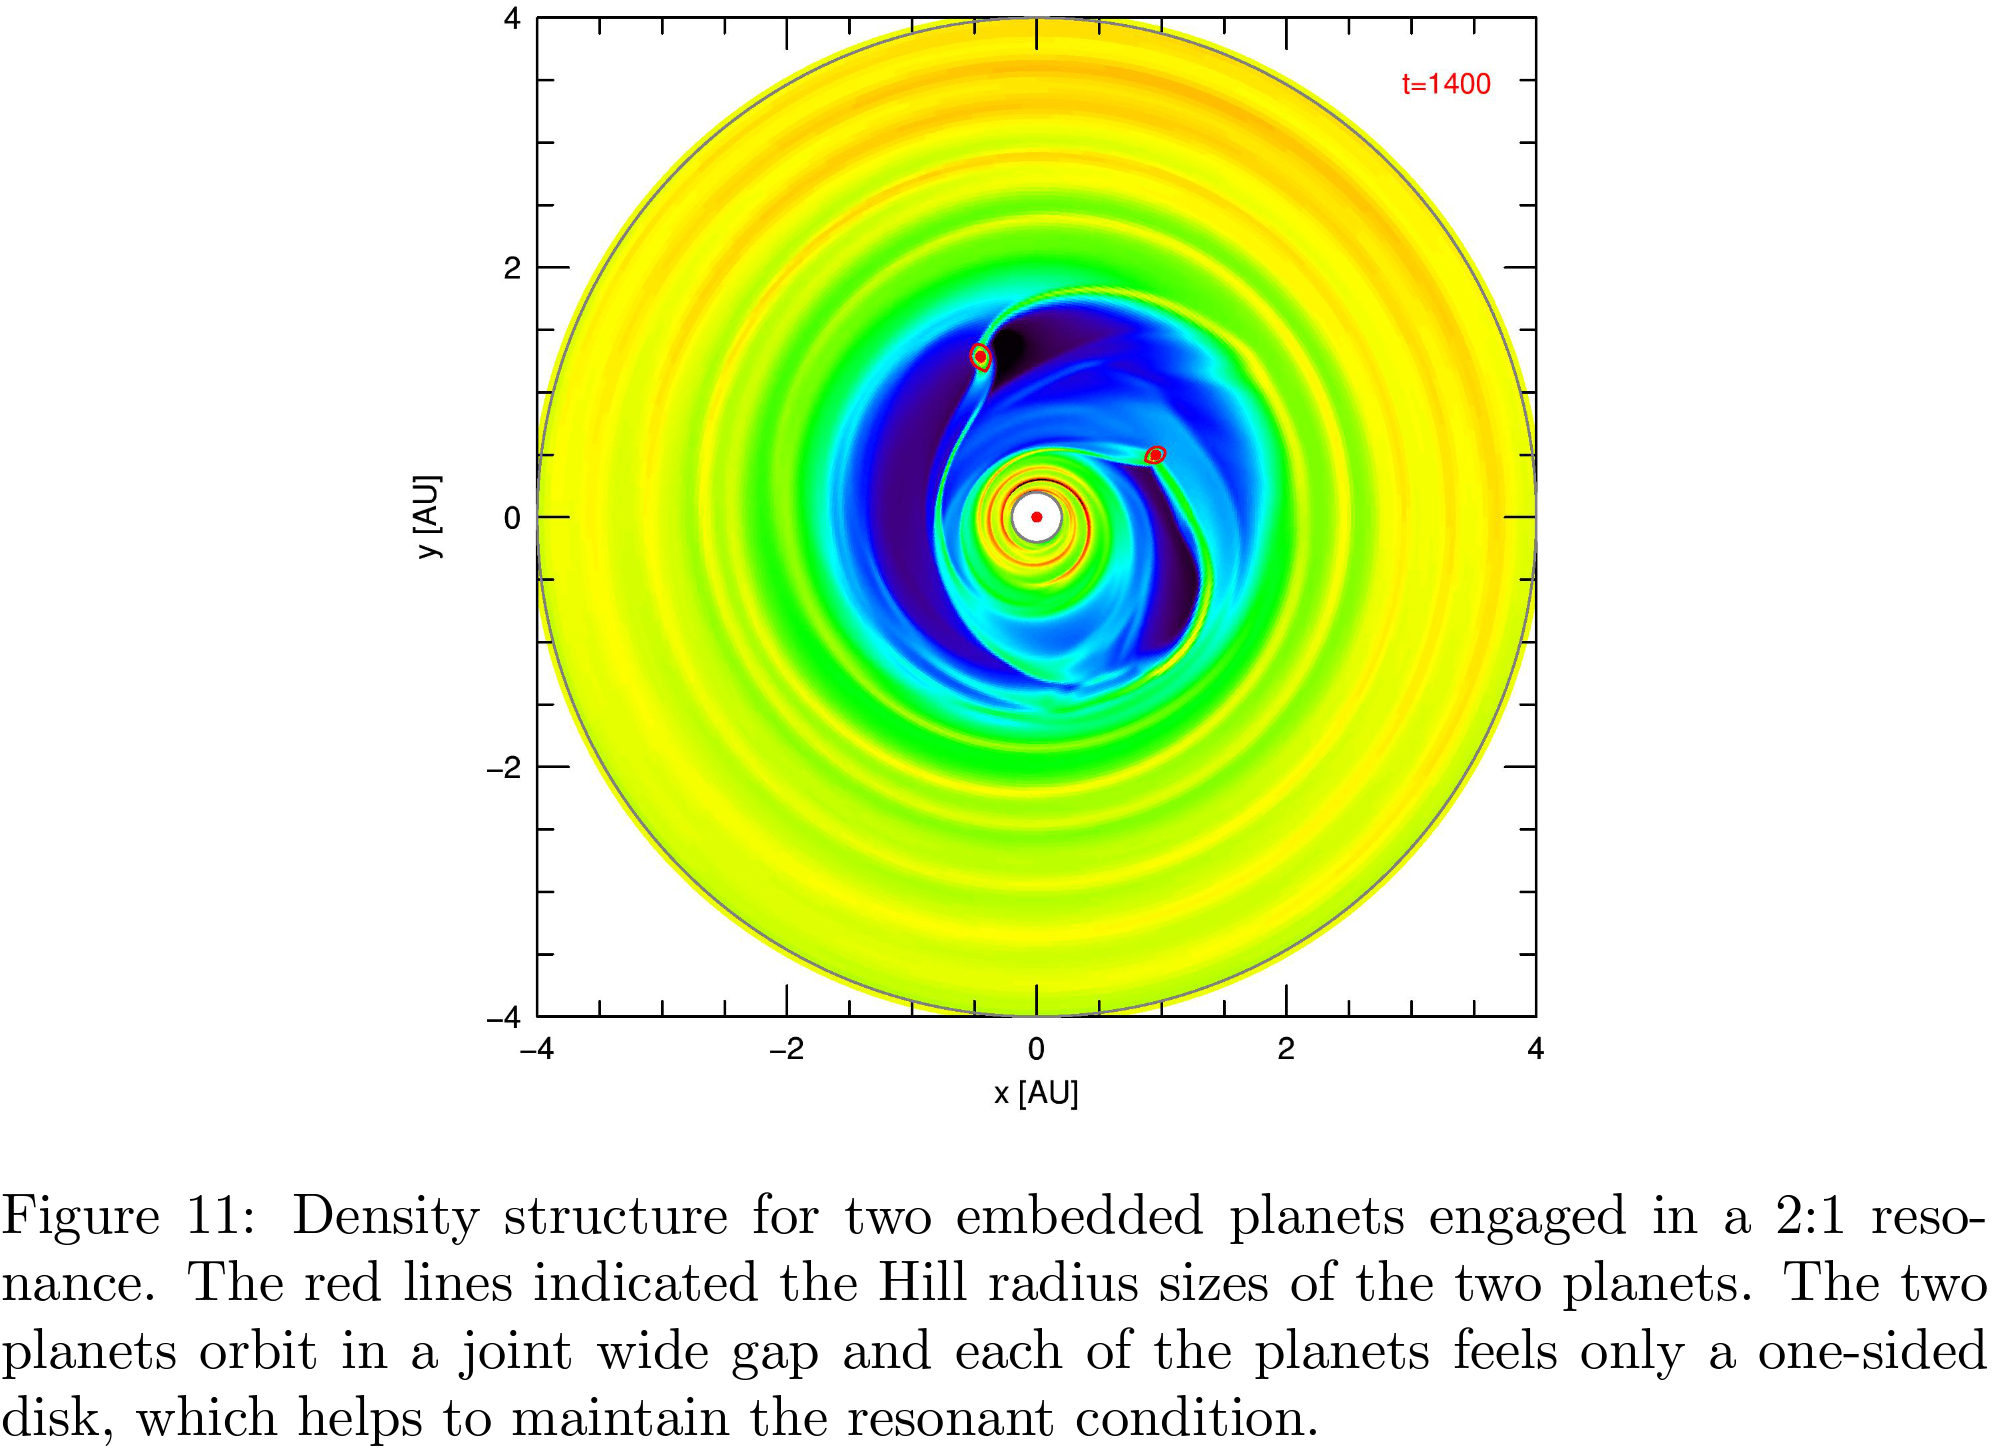
\includegraphics[trim={0cm 11cm 0 0},clip, keepaspectratio,width=0.98\textwidth]{pdres}
	\caption{Simulazione evoluzione orbite planetarie in disco di accrescimento fino a cattura in risonanza $2:1$: le regioni pi\'u dense sono in rosso. Da \cite{kley2012planet}.}\label{fig:pdres}
\end{figure}
	\end{column}
\begin{column}{0.5\textwidth}
\begin{itemize}
	\item Interazione con disco proto-planetario. 
	\item Interazione con disco residuo di planetesimi
	\item Interazione tra due o pi\'u pianeti giganti
	\item Interazione con stella in sistema di stelle binarie
	\item Interazione mareale con la stella
\end{itemize}
\end{column}
\end{columns}
\end{frame}

\begin{wordonframe}{Migrazione planetaria:}
L'osservazione di una sottopopolazione di esopianeti giganti su orbite strette, per cui sembra improbabile una formazione in loco, e la presenza di sistemi multipli in risonanza sono indicatori di evoluzione orbitale, d'altra parte nel Sistema solare fenomeni di migrazione fornisco una spiegazione all'orbita di plutone, alla presenza di numerosi oggetti della fascia di Kuiper in risonanza $3:2$ con Nettuno e al periodo di collisioni intense testimoniato da craterizzazione (Late heavy bombardment).

\end{wordonframe}